\documentclass[12pt]{article}
\usepackage[margin=2.5cm]{geometry}
\usepackage{enumerate}
\usepackage{amsfonts}
\usepackage{amsmath}
\usepackage{fancyhdr}
\usepackage{amsmath}
\usepackage{amssymb}
\usepackage{amsthm}
\usepackage{mdframed}
\usepackage{graphicx}

\begin{document}
\title{Worksheet 19 Solution}
\author{Hyungmo Gu}
\maketitle

\section*{Question 1}
\begin{enumerate}[a.]
    \item
    By the figure below, we can conclude there are 7 vertices.

    \begin{center}
    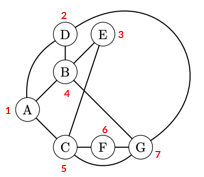
\includegraphics[width=6cm]{images/worksheet_19_q1a_solution.png}
    \end{center}

    \item
    By the figure below, we can conclude there are 11 edges.

    \begin{center}
    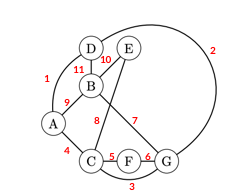
\includegraphics[width=6cm]{images/worksheet_19_q1b_solution.png}
    \end{center}

    \newpage
    \item
    By the figure below, we can conclude there are 4 vertices adjacent to G.

    \begin{center}
    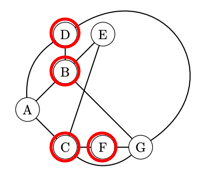
\includegraphics[width=6cm]{images/worksheet_19_q1c_solution.png}
    \end{center}

    \item
    By the figure below, we can conclude the distance between A ang G is 2.

    \begin{center}
    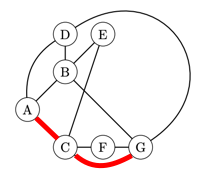
\includegraphics[width=6cm]{images/worksheet_19_q1d_solution.png}
    \end{center}

    \bigskip

    There are 2 shortest paths between A and G. One is the path from A to C to G as
    shown above, and the other is the path from A to B to G

    \begin{center}
    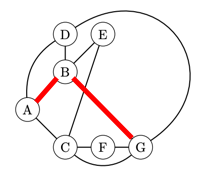
\includegraphics[width=6cm]{images/worksheet_19_q1d2_solution.png}
    \end{center}

    \begin{mdframed}
        \underline{\textbf{Correct Solution:}}

        By the figure below, we can conclude the distance between A ang G is 2.

        \begin{center}
        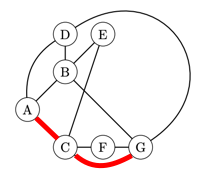
\includegraphics[width=6cm]{images/worksheet_19_q1d_solution.png}
        \end{center}

        \bigskip

        There are \color{red}3\color{black}\:shortest paths between A and G. One
        is the path from A to C to G as shown above, and the other is the path
        from A to B to G

        \begin{center}
        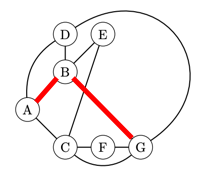
\includegraphics[width=6cm]{images/worksheet_19_q1d2_solution.png}
        \end{center}

        \color{red}
        and the last one is from A to D to G

        \begin{center}
        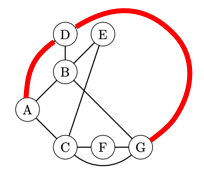
\includegraphics[width=6cm]{images/worksheet_19_q1d3_solution.png}
        \end{center}
        \color{black}
    \end{mdframed}

    \bigskip

    \textbf{Notes:}

    \begin{itemize}
     \item \textbf{Distance} is the number of edges in a shortest path.
    \end{itemize}

\end{enumerate}

\section*{Question 2}

\section*{Question 3}

\end{document}